\documentclass{article}
\usepackage{amssymb}
\usepackage{authblk}
\usepackage{caption}
\usepackage{color}
\usepackage{float}
\usepackage{graphicx}
\usepackage[utf8]{inputenc}
\usepackage{natbib}
%\usepackage[style=authoryear,backend=biber]{biblatex}

% FIXME: This is for automatic sizing of nested parentheses
%\usepackage{nath}
%\delimgrowth=1

\usepackage{nth}
\usepackage{soul}

% Big-O notation 
%\newcommand{\BigO}[1]{\ensuremath{\operatorname{O}\left(#1\right)}} % FIXME
%\newcommand{\BigO}[1]{\ensuremath{\operatorname{O}\bigl(#1\bigr)}}
%\newcommand{\bigO}[1]{\ensuremath{\mathop{}\mathopen{}\mathcal{O}\mathopen{}\left(#1\right)

\begin{document}

\title{CSCI435 Project}
\author{Paul Foster
	\thanks{Email: \texttt{pf981@uowmail.edu.au}}
	\thanks{Student Number: \texttt{3648370}}}
\affil{University of Wollongong}
\date{2013 Spring}

\maketitle

\renewcommand\abstractname{Executive Summary}
\begin{abstract}
\hl{FIXME: TODO - do not use what it is currently}
Gwynville Airport Authority has requested evaluation of some computer vision
technologies that they plan to deploy as part of their security and surveillance system.
The system should be able to count the number of people in a waiting room area based
on the image captured by a camera suitably located to `see'' the faces of passengers. Furthermore the Authority would like to recognize a speci.c group of people that are known
to be frequent users. The idea is to update their `Frequent Users'' card whenever they
are recognized in the Airport premises. In this case they intend to use a face recognition
algorithm that can learn from a dataset comprising the faces of these citizens.
\end{abstract}

Definitions: face space

\section{Introduction}
Face detection and face recognition are two actively-researched and important topics in computer vision. Both of these tasks are performed frequently and easily by humans however no current automated system exists that can be deployed effectively in an unconstrained setting \cite{sinha2006face}.

Earlier forms of facial detection and recognition involved holistic methods such as Eigenfaces\cite{turk1991eigenfaces} and Fisherfaces\cite{belhumeur1997eigenfaces}. However, more recently, local descriptors such as Local Binary Patterns (LBP)\cite{ahonen2004face} and Local Intensity Distribution (LID)\cite{nguyen2011local} have gained attention due to their efficiency and tolerance to pose and illumination changes.

Face recognition technology has significantly progressed since the proposal of the Eigenface method in 1987. Given that most individuals can only identify a few thousand people, under constrained conditions (such as fixed facial expression and lighting) and a very large number of classifications, automated face recognition can perform better than human recognition \cite{li2011handbook}.

\hl{FIXME: History of FACE DETECTION. Look at lecture notes. Good history there P.J. Phillips et.al, Overview of the face recognition grand challenge, CVPR 2005, Volume: 1, pp. 947- 954 }

There are numerous commercial and law-enforcement applications for face detection and recognition including advanced video surveillance, user authentication and suspect tracking \cite{zhao2003face}. The effectiveness of these applications rely on the efficiency and accuracy of the underlying algorithms. In this report, we will compare the efficiency and accuracy of 4 facial recognition algorithms: Eigenfaces, Fisherfaces, Local Binary Patterns (LBP) and Local Intensity Distributions (LID). We will also investigate the efficiency and performance of Haar feature-based cascade classification for face detection and discuss how these algorithms can be applied by the Gwynville Airport Authority for their security and surveillance system.


\section{Data Preparation}
The individual face data given consisted of between 9 and 14 photos each of the faces of 11 students. The images were converted to grayscale then were scaled down and cropped to 128*128. This was achieved by uniformly scaling the image such that the smaller dimension was equal to 128 pixels. The 128*128 rectangle centred at the centre of the image was then used as the cropped image. 128*128 was chosen because it was large enough to provide good results but not so large as to be computationally problematic.

For group photos, where we wanted to use the face-counting algorithm, the photo was uniformly scaled such that its area was approximately 640*480 to reduce computation.

\subsection{Training/Testing Split}
For cross validation, the student photos were split into two sets: a training set and a validation set. They were used to train the classification model and measure the performance of the model respectively. There can be no overlap in these two sets as trained images will obviously be classified correctly and will not give accurate real-world performance measures.

The proportion of the size of the training set to the size of the validation set was chosen to be \hl{FIXME:SOMETHING, look at cross validation - involves mutiple sampling. Also, maybe put this splitting into the algorithm results section as it doesn't apply to Haar}. The choice of this ratio is a balance between better classification with more training data, or more accurate performance estimates with more test data.

\hl{some\%} of the data were used to train the model and the other \hl{some\%} were used to test its performance.

\section{People Counting Algorithms}
Data Prep

\subsection{Haar}
Haar classifiers can be used to rapidly detect faces within an image in real time.

\begin{figure}[H] % FIXME: This figure wrecks page numbering
\centering
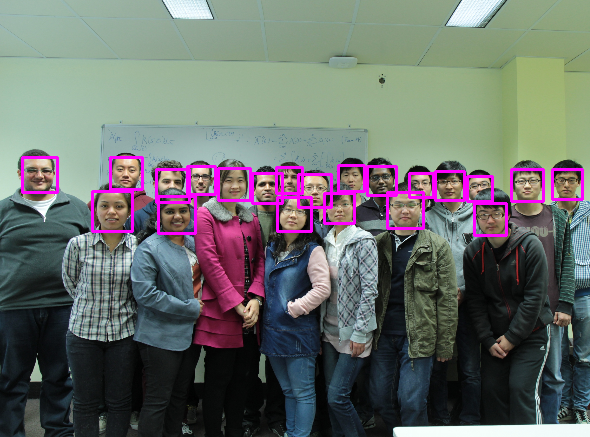
\includegraphics[width=0.7\linewidth]{./groupdetected}
\caption{Faces detected. $scaleFactor=1.01, minNeighbors=9$}
\label{fig:group}
\end{figure} % FIXME

\subsubsection{Parameter Optimisation}
There were four parameters to consider with the Haar classifier: double scaleFactor, int minNeighbors, Size minSize and Size maxSize.

I found that more faces were detected (either correctly or as false positives) as scaleFactor was increased and minNeighbors was decreased.

Starting at minNeighbors=3, I incrementally increased its value until a sufficient amount of noise (false positives) was removed. I chose the value that was the largest that still detected every face in the image. This value was 9.

Similarly for scaleFactor, I started at 1.01 and increased its value until every face was detected and there were no false positives. I found this value to be 1.017. 

I used opencv's pre-trained xml file.

I chose to leave minSize and maxSize unspecified as this would allow for detection of people at significantly varying distances to the camera.
scaleFactor=0.017; minNeighbors=9

%\begin{figure}
%\centering
%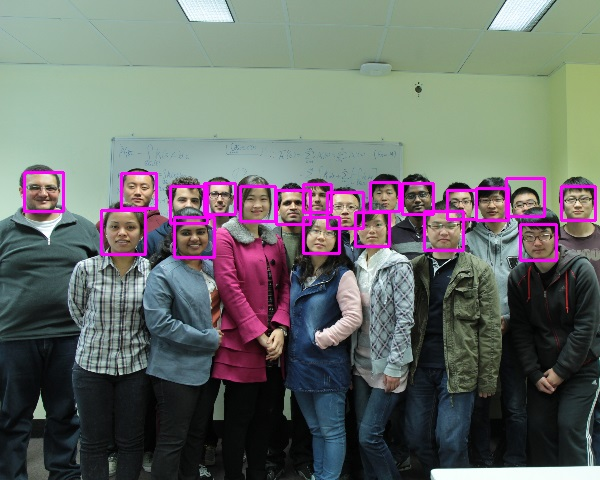
\includegraphics[width=0.7\linewidth,natwidth=10,natheight=10]{waiting_room_detected.jpg}
%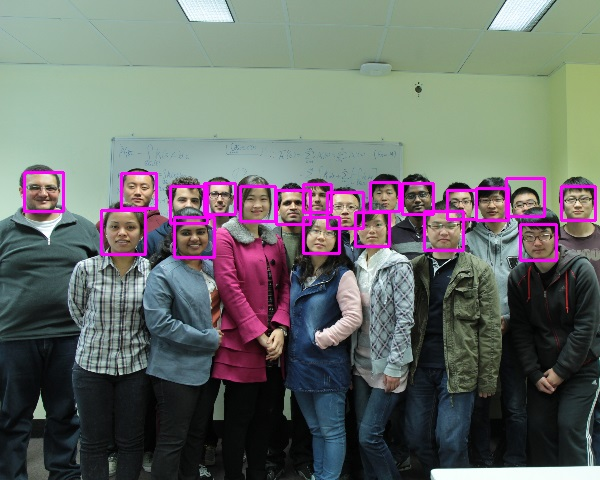
\includegraphics[width=0.1\linewidth]{waiting_room_detected.jpg} % FIXME: If this is too big it ends up restarting the page numbering
% % % %%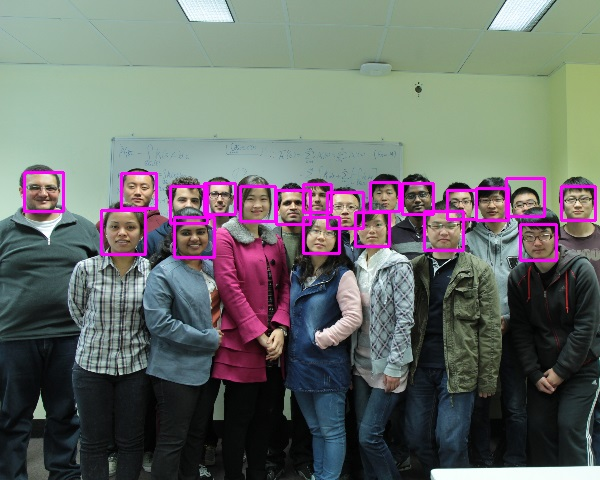
\includegraphics[scale=1]{waiting_room_detected.jpg} % FIXME: Overful hbox
%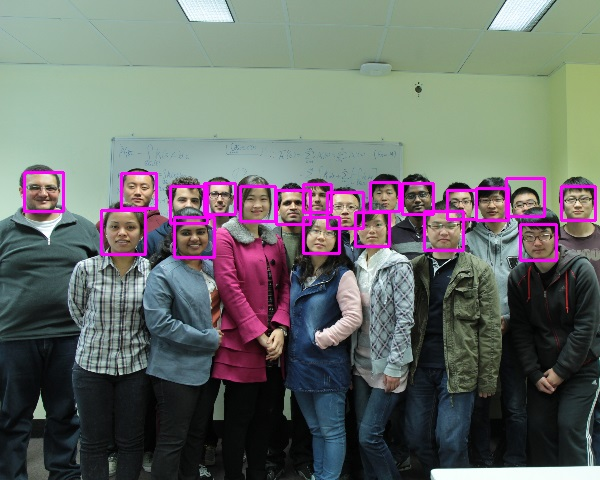
\includegraphics[width=250px,height=250px]{waiting_room_detected.jpg}
% % % %%\caption{Haar Cascade Classifier FIXME: If this is big it resets page num for some reason; FIXME: REDO - YOU HAVE CROPPED SOMEONE OUT!!!}
% % % %\label{fig:haar_cascade}
% % % %\end{figure}


%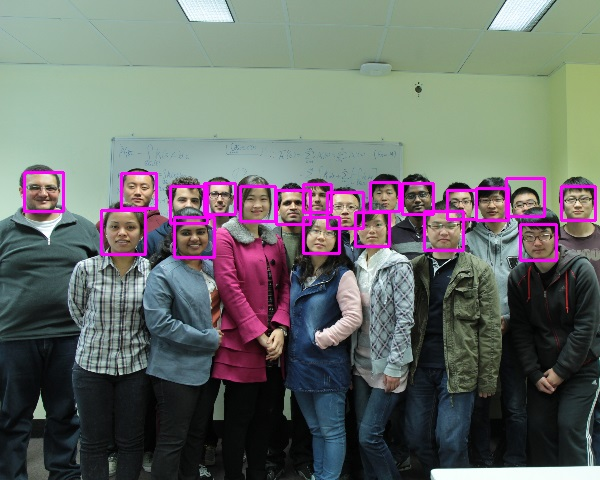
\includegraphics[width=0.7\linewidth]{waiting_room_detected.jpg}
%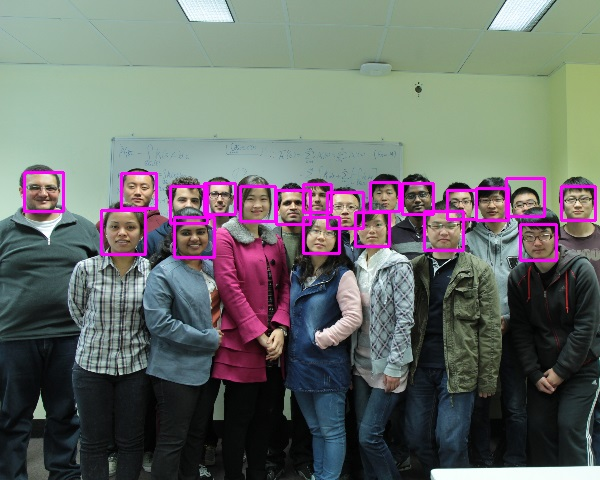
\includegraphics{waiting_room_detected.jpg} % FIXME: Too big
%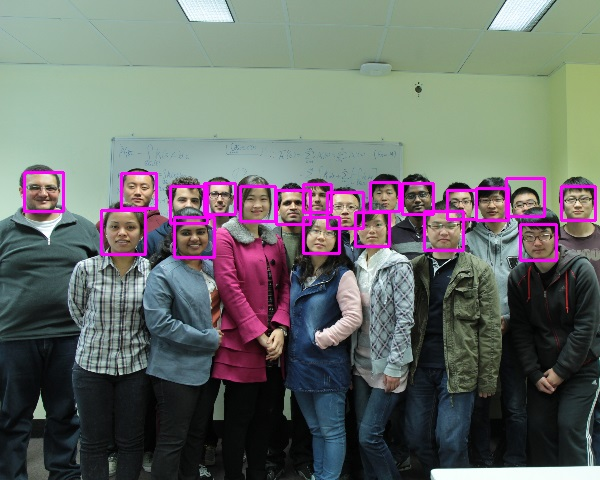
\includegraphics[scale=1]{waiting_room_detected.jpg} 

\subsection{Local Binary Patterns}
Technical description
\subsubsection{Parameter Optimisation}
Data Prep

\subsection{Comparison}
Advantages and disadvantages of each algorithm with side-by-side images after parameter optimisation


\section{Face Recognition Algorithms}
Data Prep

\subsection{Eigen Face}
If we describe the collection of all images of the face of an individual as a vector space, then we can describe every such image through a linear combination of the spanning vectors of that space.

The goal is to find the principal components of the training data, called eigenfaces. These eigenfaces form a basis for every image of this person’s face. That is, every image of this person’s face can be described as a linear combination of the eigenfaces. Furthermore, every image of this person’s face can be approximated by a linear combination of the eigenfaces with the largest eigenvalues.

\subsubsection{Calculating Eigenfaces}
Given $M$ training images with dimensions $h$*$w$, we consider each image as an $D$-dimensional vector where $D = hw$.

\vspace{12pt} \noindent Let $S$ be the set of the $M$ training images.
\begin{equation}
	S = \left\{\Gamma_1, \Gamma_2, \Gamma_3, \ldots, \Gamma_M\right\}
\end{equation}
Let $\Psi$ denote the average face of $S$. That is,
\begin{equation}
	\Psi = \frac{1}{M}\cdot\sum_{n=1}^{M}\Gamma_n
\end{equation}
Let $\Phi_i$ denote the difference between the $i$\textsuperscript{th} training face and the average.
\begin{equation}
	\Phi_i = \Gamma_i - \Psi
\end{equation}
Constructing the covariance matrix, $C \in \mathbb{R}^{D\times D}$, we get
\begin{equation}
	C = \frac{1}{M}\cdot\sum_{n=1}^{M}\Phi_n \Phi_n^T
	  = AA^T
\end{equation}
Where $A = [\Phi_1 \Phi_2 \ldots \Phi_M]$

We wish to calculate the eigenvectors ($u_1, \ldots, u_s$) of $C$. However, solving this directly is typically a computationally infeasible task.

Instead, consider the eigenvectors, $v_i$ of $A^TA$ such that $A^TAv_i=\widehat{\lambda}_iv_i$. Premultiplying by $A$ yields $AA^TAv_i=\widehat{\lambda}_iAv_i$. So clearly, $Av_i$ are the eigenvectors of $C=AA^T$.

We construct $L \in \mathbb{R}^{M\times M}$ as $L = A^T A$ such that $L_{mn} = \Phi^T_m \Phi_n$ and find the $M$ eigenvectors ($v_1, \ldots, v_k$) of $L$. These are used to computer the eigenfaces
\begin{equation}
	u_l = \sum_{k=1}^{M}v_{lk}\Phi_k \qquad k=1, \ldots, M
\end{equation}
Using this method reduces the computation from $\mathcal{O}(D)$ to $\mathcal{O}(M)$ where $M\ll D$.

To reduce the dimensionality, we keep only the eigenvectors with the largest corresponding eigenvalue. These vectors account for the most variation in the images. There are several ways of determining how many vectors to keep, but we chose to keep the eigenvalues that accounted for 90\% of the sum of the eigenvalues. \hl{FIXME: CHECK THIS what does OPENCV do?}

\subsubsection{Using Eigenfaces for Face Recognition}
To classify a face image $\Gamma$, we project it into its "face space" using $\omega_k = u^T_k(\Gamma - \Psi)$, for $k = 1, \ldots, M^\prime$.

Let $\Omega^T = [\omega_1, \ldots, \omega_{M^\prime}]$ and let $\Omega_k$ denote the vector describing the $k$th face class.

We wish to find $k$ that minimises $\epsilon_k = \|(\Omega - \Omega_k)\|$. If such an $\epsilon_k$ is above some threshold $\theta_\epsilon$, then we say the face is unknown. Otherwise we classify the face as the $k$th class.

\subsubsection{Parameter Optimisation}
Data Prep

\subsection{Fisherfaces}
The main advantage of this method is that it is invariant to different light sources. Extensive experimental results show that Fisherface has lower error rates than eigenface on the havard and yale face detection databases. \hl{(See the abstract of the pdf)}.

The Fisherfaces method recognises that variance among faces in the database may come from distortions such as illumination changes or facial expressions. Sometimes these variations within a face class are larger than the variations between classes of faces.

\hl{Although this method has advantages when subject to different lighting conditions, this advantage is not really applicable to our purposes as the camera will likely be uniformly lit. (Maybe it will be important if it is sometimes lit by natural light and sometimes lit by artificial light depending on the time of day.}

Like Eigenfaces, the Fisherfaces algorithm reduces the dimensionality of the problem. It does so in a way the preserves the linear separability of the classes. We wish to choose \hl{$W$} such that the ratio of the between-class scatter and within-class scatter is maximised. We define the between-class scatter matrix as $S_B = \sum_{i=1}^{c}N_i(\mu_i - \mu)(\mu_i - \mu)^T$ and the within-class scatter matrix as  $S_W = \sum_{i=1}^{c}\sum_{x_k\in X_i}(x_k - \mu_i)(x_k - \mu_i)^T$. Where $u_i$ is the mean image of class $X_i$ and $N_i$ is the number of samples in class $X_i$.

$S_W$ is either singular or non-singular. If it is singular, choose $W_{opt}$ as the matrix with orthonormal columns such that $\frac{|W^TS_BW|}{|W^TS_WW|}$ is maximised. That is
\begin{equation}
	W_{opt} = arg\ max_W \frac{|W^TS_BW|}{|W^TS_WW|} = [w_1\ w_2\ \ldots\ w_m]
\end{equation}
Where $w_i$ is the $i$th generalised eigenvector of $S_B$ and $S_W$ corresponding to the $m$ largest generalised eigenvalues ($\lambda_1, \ldots, \lambda_m$). So we have
\begin{equation}
	S_Bw_i = \lambda_iS_Ww_i,\quad i=1, \ldots, m
\end{equation}
However, in face recognition problems, $S_W$ is always singular \cite{belhumeur1997eigenfaces}. To solve this problem, we use PCA to project the image to a lower dimensional space such that $S_W$ is nonsingular. We wish to find $W_{opt}^T$ such that $W_{opt}^T = W_{fld}^TW_{pca}^T$ where $W_{pca} = arg\ max_W|W^TS_TW|$ and $W_{fld} = arg\ max_W\frac{|W^TW_{pca}^TS_BW_{pca}W|}{|W^TW_{pca}^TS_WW_{pca}W|}$.

\subsubsection{Parameter Optimisation}
Data Prep

\subsection{Local Binary Patterns}
The LBP descriptor describes a pixel as an $P$-bit binary number based on the values of $P$ points on the circumference of a circle of radius $R$ centred at the pixel. This number becomes its label.

Because LBP converts pixels to an binary number, computations can be done with integer arithmetic which results in significant performance advantages over the other methods which use floating-point arithmetic.

We will define a uniform pattern to be a binary pattern containing at most two bitwise transitions from 0 to 1 or 1 to 0 when the pattern is traversed circularly. For example $01110000$ and $00000000$ are uniform whereas $01101000$ and $00110011$ are not.

Let $(P, R)$ denote the pixel neighbourhood of $P$ evenly-spaced points on the circumference of a circle of radius $R$.

Let $LBP^{u^2}_{P,R}\cdot$ denote the LBP operator in a $(P, R)$ neighborhood using only uniform patterns ($u^2$) and labelling all remaining patterns with a single label.
% FIXME: http://www.scholarpedia.org/article/Local_Binary_Patterns


\hl{$n$ neighboring pixels 
YOU HAVEN'T EXPLAINED HOW TO CALCULATE LBP OPERATOR
The image is equally split into $X$ columns and $Y$ rows. Each of these regions is given a weight.}
\subsubsection{Training LBP}
Training involves obtaining a description for each training image.

Each of the training images are trained in the following way. Each pixel, $p$, is given a classification of $LBP_{P,R}^{u^2}(p)$. The image is split evenly into $X$ columns and $Y$ rows and the histogram of the local binary patterns of its constituent pixels is determined. These histograms are then normalised.

Our description for the image consists of a spacial histogram: $X\cdot Y$ histograms, which each correspond to a region of the image, appended together.

\subsubsection{Face Recognition Using LBP}
Given an unclassified image $I$, its description (a spacial histogram) is determined using the previous method. For each of the training images $I^{(i)}$, the chi-squared distance between the training image's spacial histogram, $H^{(i)}$, and the unclassified image's histogram, $H$, is calculated.
We classify the image as the class of the closest training image. That is,
\begin{equation}
	class\{I\} = class\{I^{(k)}\}
\end{equation}
where $I_k$'s spacial histogram has the smallest chi-squared distance to $I$'s spacial histogram. That is, $k$ is chosen such that
\begin{equation}
	\chi^2(H, H^{(k)}) = \sum_{j=1}^{n}\frac{(H_j - H^{(k)}_j)^2}{H_j + H^{(k)}_j}
\end{equation}
is minimised, where $H^{(k)}_j$ denotes the $j$th element of the spacial histogram $H^{(k)}$.

We add the additional constraint that $class\{I\}$ will be \textit{unknown} if the distance is not within some threshold, $\theta$. That is,
\begin{equation}
	\chi^2(H, H^{(i)}) > \theta \Rightarrow class\{I\} = unknown
\end{equation}

\subsubsection{Additional Notes}
Many enhancements have been proposed for LBP. These include considering neighbours that lie on an ellipse rather than a circle, non-rectangular regions, weighted regions, regions of different sizes and overlapping regions \cite{belhumeur1997eigenfaces}. However, we will only be testing the method specified above.


\subsubsection{Parameter Optimisation}
Data Prepsssss

\subsection{Local Intensity Distribution}
\hl{Insert diagram to illustrate what neighboring pixels are in LID. Do the same for LBP.

Local Intensity Distribution (LID) descriptors can be used to describe the features of an intensity image by capturing the distribution of local intensity differences. Similar to LBP descriptors, LID descriptors are insensitive to illumination changes} \cite{nguyen2011local}.

\subsubsection{The LID Descriptor}
Let $I(x,y) : \mathbb{Z}^2 \rightarrow \mathbb{R}$ denote the intensity image of an image with $N$ pixels and let $p = (x,y) \in \mathbb{Z}^2$ be an arbitrary point in the domain of $I$. We define $LID_{N,R}(p) : \mathbb{Z}^2 \rightarrow \mathbb{R}^N$ as
\begin{equation}
   % \label{simple_equation}
   LID_{N,R}(p) = \langle d(p_1,p), \ldots, d(p_n,p)\rangle
\end{equation}
where $d(p_i,p) = I(p_i) - I(p)$ and $p_i = (x_i, y_i) \in \mathbb{Z}$ is such that $max\{|x_i - x|, |y_i - y|\} = R$. % FIXME: There must be a better way to describe this rectangle (perimeter) than using this max.

\subsubsection{Training The Images}
% FIXME: I suspect that if you use spacial histograms instead of SIFT you will get better results

\subsubsection{Alternative Methods for LID Face Detection}
\label{sec:alternativeLID}

\subsubsection{Parameter Optimisation}
Data Prep

\subsection{Comparison}
Advantages and disadvantages of each algorithm with side-by-side images after parameter optimisation

\subsubsection{Why Eigenfaces and Fisherfaces Performed Worse Than Expected}
Both the Eigenfaces and Fisherfaces methods are reported to have a \hl{some\%} rate of accuracy \hl{Some citation} however our testing showed only \hl{x\%} and \hl{y\%} respectively. I believe the reason for this discrepancy is because both of these methods are sensitive to pose \cite{turk1991eigenfaces}\cite{belhumeur1997eigenfaces}. The reported good performance of these methods have been on databases which contained faces with only one frontal view. The images we have tested with in this report have had very varying poses (See figure~\ref{fig:pose}). This may be the cause of these algorithms poor performance.

Although the Eigenfaces and Fisherfaces implementations used in this report are sensitive to variance of pose, there exist modern modifications to these algorithms to reduce that sensitivity \cite{jaiswal2012local}.
\begin{figure}[H]
\centering
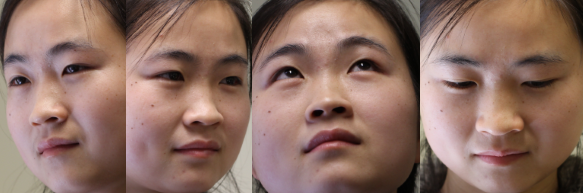
\includegraphics[width=0.7\linewidth]{./pose}
\caption{Images showing variation in pose in the dataset}
\label{fig:pose}
\end{figure} % FIXME

\subsubsection{Why The LID Implementation Performed so Poorly}
Overall, the LID algorithm for face recognition performed very poorly. Of the four algorithms it by far performed the worst in terms of correctly identifying faces. \hl{Show an image of all the training faces of a person with the sift keypoints marked}. I believe that this is due to the SIFT keypoints detecting significantly different sections of the face for each image of the same person. This results in comparing LID descriptors of different parts of the face. As we were not comparing the descriptors for the same part of the face, the histogram comparisons were not an accurate measure of the dissimilarity of the faces.

I believe the alternative method of computing spacial histograms, as outlined in section~\ref{sec:alternativeLID}, would result in much better performance as we would be comparing corresponding regions of images in the same way LBP does.


\section{Recommendation}
conc

When implementing the airline actual thingo, you should constantly add to your training data.
So when you see a person and you confidently classify them as known, add that image to the training data.
If you see the same unknown face, calculate its characteristics and make it known. This is what they want because then they would be able to tell who is frequent without having to manually train.
The implementation you are looking for would be to use the face counter and then send each face into the second algorithm which will attempt to identify them.
It is critical that the camera have a frontal face view as the training data for the Haar cascade classifier was frontal faces.


\section{Conclusion}
All these faces were trained with the same illumination and facial hair etc on the same day. It will likely not perform well on images of different illumination.

We found that eigen and fisher took significantly longer to train and compute

FIXME: The VERY LARGE DISTANCES for eigen and fisher could be due to the variation in pose. This is why it performs significantly poorer than in the papers as they dealt with fixed pose

Our results found that both the Eigenfaces and Fisherfaces algorithms performed very poorly in terms of performance. When tuning parameters, we had the problem that if we reduced to too few dimensions, it would classify things incorrectly. On the other hand, if we chose too many dimensions, the distances between classifications would be far too large - normally in the thousands (rephrase - explain maths - higher dimensionality=bigger distances).

Because the distances were so large, it tended to misclassify confidently rather than classify as unknown.

This could be due to the face that both algorithms are intolerant of variations in pose. When one looks at the images, all individuals hand different head rotations and angles which may explain the poor performance compared to experiments in other papers\cite{belhumeur1997eigenfaces}. There are several modifications to the algorithm that would make this method deal with pose variation such as CITATION.

Notes on our training data: Variations in pose, no variation in lighting, some people put on glasses, variations in facial expression

FIXME: Explain what happened when you reduced the resolution to 128*128: Fisher and eigen sped up immensely and lbp performed more poorly.


\bibliographystyle{plain}
\bibliography{references}



\end{document}
% FIXME: There is a problem: The page numbers restart in the middle Just hack it to work - they only want the pdf :-( Don't know why
% FIXME: For training, we don't really test false positives. We could give it some faces not in the dataset.
% FIXME: Look at http://people.wku.edu/qi.li/teaching/595_BA/ba16_Eigenface.pdf for cross-validation in determining the best split
% If you run out of space: http://www.terminally-incoherent.com/blog/2007/09/19/latex-squeezing-the-vertical-white-space/
% You could talk about the evolution of LBP - originally just 8 neighbors then circle then ellipse. Originally didn't exclude non-uniform binary patterns. The regions do not have to be rectangular or the same size and do not have to cover the whole image - could even overlap.
% THIS IS A REALLY GOOD LBP PAPER - might illuminate some info for LID: http://web.ing.puc.cl/~asoto/papers/Maturana-09.pdf